%!TEX TS-program = xelatex
\documentclass[a4paper,10pt,twocolumn,oneside]{article}
\setlength{\columnsep}{10pt}  
\setlength{\columnseprule}{0pt}      

\usepackage{amsthm}	
\usepackage{amssymb}
%\usepackage[margin=2cm]{geometry}
\usepackage{fontspec}
\usepackage{color}
\usepackage[x11names]{xcolor}
\usepackage{listings}	
\usepackage[Glenn]{fncychap}
\usepackage{fancyhdr}
\usepackage{graphicx}
\usepackage[export]{adjustbox}								%Graphic
\usepackage{enumerate}
\usepackage{changepage}
\usepackage{titlesec}
\usepackage{amsmath}
\usepackage{codebook}
\usepackage{verbatim}
\usepackage[CheckSingle, CJKmath]{xeCJK}
% \usepackage{CJKulem}

%\usepackage[T1]{fontenc}
\usepackage{amsmath, courier, listings, fancyhdr, graphicx}
\topmargin=0pt
\headsep=5pt
\textheight=780pt
\footskip=0pt
\voffset=-40pt
\textwidth=545pt
\marginparsep=0pt
\marginparwidth=0pt
\marginparpush=0pt
\oddsidemargin=0pt
\evensidemargin=0pt
\hoffset=-42pt

%%%%%%%%%%%%%%%%%%%%%%%%%%%%%

\setmainfont{Consolas}	
\setmonofont{Monaco}
%\setCJKmainfont{Source Han Sans}
% \setCJKmainfont{Consolas}
%\setmainfont{sourcecodepro}
\XeTeXlinebreaklocale "zh"
\XeTeXlinebreakskip = 0pt plus 1pt
\setcounter{secnumdepth}{3}

%%%%%%%%%%%%%%%%%%%%%%%%%%%%%
\makeatletter
\lst@CCPutMacro\lst@ProcessOther {"2D}{\lst@ttfamily{-{}}{-{}}}
\@empty\z@\@empty
\makeatother
\lstset{											% Code
language=C++,										% the language of the code
basicstyle=\ttfamily, 						% the size of the fonts that are used for the code
%numbers=left,										% where to put the line-numbers
numberstyle=\footnotesize,						% the size of the fonts that are used for the line-numbers
stepnumber=1,										% the step between two line-numbers. If it's 1, each line  will be numbered
numbersep=5pt,										% how far the line-numbers are from the code
backgroundcolor=\color{white},					% choose the background color. You must add \usepackage{color}
showspaces=false,									% show spaces adding particular underscores
showstringspaces=false,							% underline spaces within strings
showtabs=false,									% show tabs within strings adding particular underscores
frame=false,											% adds a frame around the code
tabsize=2,											% sets default tabsize to 2 spaces
captionpos=b,										% sets the caption-position to bottom
breaklines=true,									% sets automatic line breaking
breakatwhitespace=false,							% sets if automatic breaks should only happen at whitespace
escapeinside={\%*}{*)},							% if you want to add a comment within your code
morekeywords={*},									% if you want to add more keywords to the set
keywordstyle=\bfseries\color{Blue1},
commentstyle=\itshape\color{Red4},
stringstyle=\itshape\color{Green4},
literate={\ \ }{{\ }}1
}

\university{1}{Saratov State University}{SSU.png}
\team{ZAVRS}{Eremenko, Utaliev, Yanchenko}
\contest{Contest name}{Contest Date}

%%%%%%%%%%%%%%%%%%%%%%%%%%%%%

\begin{document}
\maketeampage

\pagestyle{fancy}
\fancyfoot{}
%\fancyfoot[R]{
\includegraphics[width=12pt]{SSU.png}}
\fancyhead[L]{Saratov State University: Eremenko, Utaliev, Yanchenko}

\fancyhead[R]{\thepage}
\renewcommand{\headrulewidth}{0.4pt}
\renewcommand{\contentsname}{Contents} 
\scriptsize
\begingroup
\let\clearpage\relax
% \tableofcontents
\endgroup
\tableofcontents
%%%%%%%%%%%%%%%%%%%%%%%%%%%%%
% \newpage

\section{Basic}
\code{Fast I/O}{basic/fastio.cpp}
\code{Pragma optimization}{basic/pragma.cpp}
\code{Hash Function}{basic/hash.cpp}
\code{Random Double}{basic/rnd\_ld.cpp}

\section{Math}
\codewithtext{Berlekamp Messey}{math/bm.cpp}{Store the linear recurrence relation of form $A_{t+n} = \sum \limits_{i = t}^{t+n-1} \mathit{coef}_i \cdot A_i$, linear\_recurrence works in $O(n \cdot sz + sz \log mod)$, operator [] is $n^2 \log i$}
\codewithtext{Simplex Algorithm}{math/simplex.cpp}{maximize $\mathbf{c}^T\mathbf{x}$ subject to $A\mathbf{x} \leq \mathbf{b}$ and $\mathbf{x} \geq 0$. Returns $-\infty$ if infeasible and $\infty$ if unbounded.}
\code{Integration}{math/integration.cpp}
\code{Simulated Annealing}{math/annealing.cpp}
\code{Gauss}{math/gauss.cpp}
\code{Iteration}{math/iteration.cpp}
\codewithtext{Tridiagonal Matrix Algorithm}{math/tridiag.cpp}{$a_{i}x_{i-1}+b_{i}x_{i}+c_{i}x_{i+1}=d_{i}$}

\section{Number Theory}
\code{FFT}{nt/fft.cpp}
\code{NTT}{nt/ntt.cpp}
\code{Online FFT}{nt/online-fft.cpp}
\code{FWHT}{nt/fwht.cpp}
\code{Extended Euclid}{nt/exgcd.cpp}
\tex{Burnside Lemma}{nt/burnside.tex}
\tex{Lucas Theorem}{nt/lucas.tex}
\code{Phi and Mobius}{nt/phimu.cpp}
\code{CRT}{nt/crt.cpp}
\code{Pollard Rho}{nt/pollard.cpp}
\code{Miller Rabin}{nt/miller.cpp}
\code{Primitive Root}{nt/primitive.cpp}
\code{Discrete Root}{nt/discrete\_root.cpp}
\tex{Partitions}{nt/partition.tex}
\codewithtext{Smallest Multiple Modulo}{nt/smallest\_modulo.cpp}{Returns the smallest non-negative integer $x$ s.t $l \le ax \mod p \le r$; IMPORTANT : $0 \le a < p$, $0 \le l \le r < p$, $p$ is not necessarily prime}
\codewithtext{Diophantine Equations}{nt/diophantine.cpp}{solutions to $ax + by = c$ where $x \in [xlow, xhigh]$ and $y \in [ylow, yhigh]$; returns \{cnt, leftsol, rightsol, gcd of a and b\}}
\codewithtext{Floor Sum of Arithmetic Progression}{nt/floorsum.cpp}{$\sum_{i=0}^{n-1} \lfloor \frac{ai + b}{m} \rfloor$}
\code{Stern-Brocot Tree}{nt/stern-brocot.cpp}
\codewithtext{Lattice Points Below Line}{nt/lattice\_points.cpp}{Number of integer points $(x;y)$ such for $0 \leq x < n$ and $0 < y \leq \lfloor k x+b\rfloor$}

\section{Graph Theory}
\code{Biconnected Components}{graph/bicon.cpp}
\code{2-SAT}{graph/twosat.cpp}
\codewithtext{Directed MST}{graph/arbor.cpp}{$O(E \log V)$, returns the list of the edge indices or an empty list if there is no answer, INF should be greater than the maximum edge weight}
\code{Maximum Clique}{graph/maxclique.cpp}
\tex{Counting Labeled Graphs}{graph/labeled\_graphs.tex}
\tex{Kirchoffs Theorem}{graph/kirghoff.tex}
\tex{Tuttes Theorem}{graph/tutte.tex}
\tex{Matching Duals}{graph/matching\_dual.tex}

\section{Flows}
\code{Dinics Algorithm}{flows/dinics.cpp}
\code{MCMF}{flows/mcmf.cpp}
\codewithtext{MCMF with Potentials}{flows/mcmf\_potentials.cpp}{call init\_dag() or init\_fb() (depending on if your graph is dag or not) before running calc()}
\tex{L-R Flow}{flows/lrflow.tex}
\code{Gomory-Hu Tree}{flows/gomoryhu.cpp}
\code{Stoer Wagner Algorithm}{flows/stoer-wagner.cpp}
\code{Hungarian Algorithm}{flows/hungarian.cpp}
\code{Blossom Algorithm}{flows/blossom.cpp}
\code{Blossom Algorithm Weighted}{flows/blossom-weighted.cpp}
\code{Minimum Cost Circulation}{flows/mincost\_circ.cpp}

\section{Data Structures}
\code{Segment Tree Beats}{ds/beats.cpp}
\code{Centroid Decomposition}{ds/centroid.cpp}
\code{HLD}{ds/hld.cpp}
\code{LCT}{ds/lct.cpp}
\code{Explicit Treap}{ds/treap.cpp}
\code{Ordered Set}{ds/pbds.cpp}

\section{Strings}
\tex{String Matching with FFT}{strings/fft\_match.tex}
\codewithtext{Suffix Array}{strings/suffix\_array.cpp}{Don't forget to modify the string to avoid cyclic comparisons if needed}
\code{Suffix Array Linear}{strings/sais.cpp}
\code{Suffix Tree}{strings/suffix\_tree.cpp}
\code{Palindromic Tree}{strings/eertree.cpp}
\code{Manachers Algorithm}{strings/manacher.cpp}
\code{Prefix Automaton}{strings/prefix\_automaton.cpp}
\code{Aho-Corasick}{strings/aho.cpp}
\code{Lyndon Decomposition}{strings/lyndon.cpp}
\code{Repetitions}{strings/repetitions.cpp}

\section{DP}
\code{Dynamic CHT}{dp/cht.cpp}
\code{Li Chao Tree}{dp/lichao.cpp}
\code{D\&C Optimization}{dp/dnc.cpp}
\codewithtext{Knuth Optimization}{dp/knuth.cpp}{Достаточное условие: 1. $C_{ac}+C_{bd}\le C_{ad}+C_{bc}$, 2. $C_{bc}\le C_{ad}$, при всех $a\le b\le c\le d$.}
\codewithtext{Slope Trick}{dp/slope.cpp}{You are given an array, each operation you are allowed to increase or decrease an element's value by $1$. Find the minimum number of operations to make the array strictly increasing.}
\codewithtext{1D1D}{dp/1d1d.cpp}{$dp_i=\min \limits_{j<i} dp_j + b_j \cdot a_i$, $\forall i<j: a_i < a_j, b_i > b_j$; Достаточное условие: $C_{ac}+C_{bd}\le C_{ad}+C_{bc}$, при всех $a\le b\le c\le d$.}

\section{Geometry}
\code{Circle Circle Area}{geometry/circle\_circle\_area.cpp}
\code{Circle Line Intersection}{geometry/circle\_line.cpp}
\code{Circle Circle Intersection}{geometry/circle\_circle.cpp}
\code{Tangent Lines of Two Circles}{geometry/tangents\_circles.cpp}
\code{Minkowski Sum}{geometry/minkowski.cpp}
\code{Convex Hull 3D}{geometry/convex3d.cpp}
\tex{Closest Pair of Points}{geometry/closest\_pair.tex}
\tex{Delaunay Triangulation}{geometry/delaunay.tex}
\tex{Voronoi Diagram}{geometry/voronoi.tex}
\code{Half Plane Intersection}{geometry/halfplane.cpp}
\code{Point in Convex Polygon}{geometry/point\_in\_convex.cpp}
\code{SVG}{geometry/svg.cpp}

\section{Game Theory}
\code{Nim Multiplication}{games/nim.cpp}

\section{Miscellaneous}
\code{Josephus Problem}{misc/josephus.cpp}
\code{Knight Moves in Infinity Grid}{misc/knight.cpp}
\code{Poker Hands Comparison}{misc/poker.cpp}
\tex{Matroid Intersection}{misc/matroid.tex}
\code{Python Libs}{misc/python\_libs.py}

\setlength{\parindent}{0cm}
\section{Other}
\tex{Комбинаторика}{other/combinatorics.tex}
\tex{Теория чисел}{other/number-theory.tex}
\tex{Геометрия}{other/geometry.tex}
\tex{Графы}{other/graphs.tex}
\tex{Формулы}{other/other.tex}
\tex{Полезные числа}{other/table.tex}

%\begin{figure}[h!b]
\includegraphics[height=\textheight,keepaspectratio=true]{misc/hexagonal.ps}
%\end{figure}

\end{document}
